\chapter{Problem description}

\textit{(TODO:Pending an introduction to radio astronomy)}
\section{Radio Astronomy topics related to observations scheduling problem}
\subsubsection{Sensitivity}
\label{sec:sens}
The observation total RMS noise could be accumulated over different observation sessions, only if all the observations are done over the same target, with the same observational setup (i.e., same correlator configuration and observing frequency). The accumulated RMS noise over the time for a given setup is known as \textit{sensitivity}.

The RMS noise for multiple observations $\sigma$ is accumulated as shown in equation \ref{eq:rms-noise}.
\begin{equation}
\label{eq:rms-noise}
\sigma = \frac{\sqrt{\sum_{i=1}^M \sigma_i^2}}{M}
\end{equation}
where $M$ is the number of SBs and $\sigma_i$ is the RMS noise for a single
execution of an SB, calculated differently depending of the type of observation.
For interferometric observations the sensitivity is given by equation \ref{eq:sensitivity-interferometry}.
\begin{equation}
\label{eq:sensitivity-interferometry}
\sigma_i^{INT} = \frac{T_{sys}^i}{\eta_Q \sqrt{N_{INT}^i(N_{INT}^i-1)(\Delta\nu)\tau^i}}
\end{equation}
where $T_{sys}^i$ is the system temperature, $\eta_Q$ is the correlator sensitivity,
$N_{INT}^i$ is the number of antennas, $\Delta\nu$ is the bandwidth, and $\tau^i$ is
the integration time. All the quantities with the $i$ superscript are specific for the $i$-th
observation.

For single-dish observations
\begin{equation}
\sigma_i^{SD} = \frac{\alpha T_{sys}^i \sqrt{N_{SD}^i}}{\sqrt{(\Delta\nu)\tau^i}}
\end{equation}
where $\alpha$ is a numerical factor that depends on the scanning mode ($\sim 1$ for OTF,
$\sim \sqrt{2}$ for switched observations).

The RMS values are expressed in degrees Kelvin. To convert them to flux units, they are multiplied by the factor $2k/A_e$ where $k$ is the Boltzmann constant and $A_e$ is the antenna effective aperture.

These equations do not cover the case of the combined array, where the antennas in the array have different sizes, nor cover the cases where the bandwidth has been changed (multi-resolution modes, etc.).

\subsubsection{Angular resolution}
\label{sec:angular-res}
A first order approximation of the resolution that can be attained with a give
array configuration is $\theta = \lambda / l_{max}$ where $l_{max}$ is the maximum
baseline in the array.

\textit{TODO: Try to get the derivation of the angular resolution of an array}

\subsection{Weather considerations}

The Earth atmosphere is a layer of gases surrounding the solid mass of Earth. This layer of gases is maintained in this position due the gravitational effect of the solid mass. Most of the Earth's atmosphere is composed by Nitrogen and Oxygen used by most of the micro-organisms for respiration and some carbon dioxide used by most of the plants and other organism for photosynthesis,	also it serves as protection of ultraviolet radiation for the living organisms. Most of the mass (around $80\%$) of the atmosphere and almost all the weather phenomenon occurs in the lowest layer of the Earth's atmosphere, the \textit{Troposphere}.

The troposphere is extending from Earth's surface to 7 to 10 km of altitude, the temperature decreases with altitude in this layer, clouds form and convection can be significant. The troposphere is composed mainly of $N_2$, $O_2$, trace gases such as water vapor, $N_2O$ and $CO_2$, and particles such as liquid water and dust in clouds. Generally, the troposphere become increasingly opaque with increasing frequency as shown in figure \ref{fig:atmospheric-opacity}, mostly due the absorption by $O_2$ and $H_2O$.

\begin{figure}[htbp]
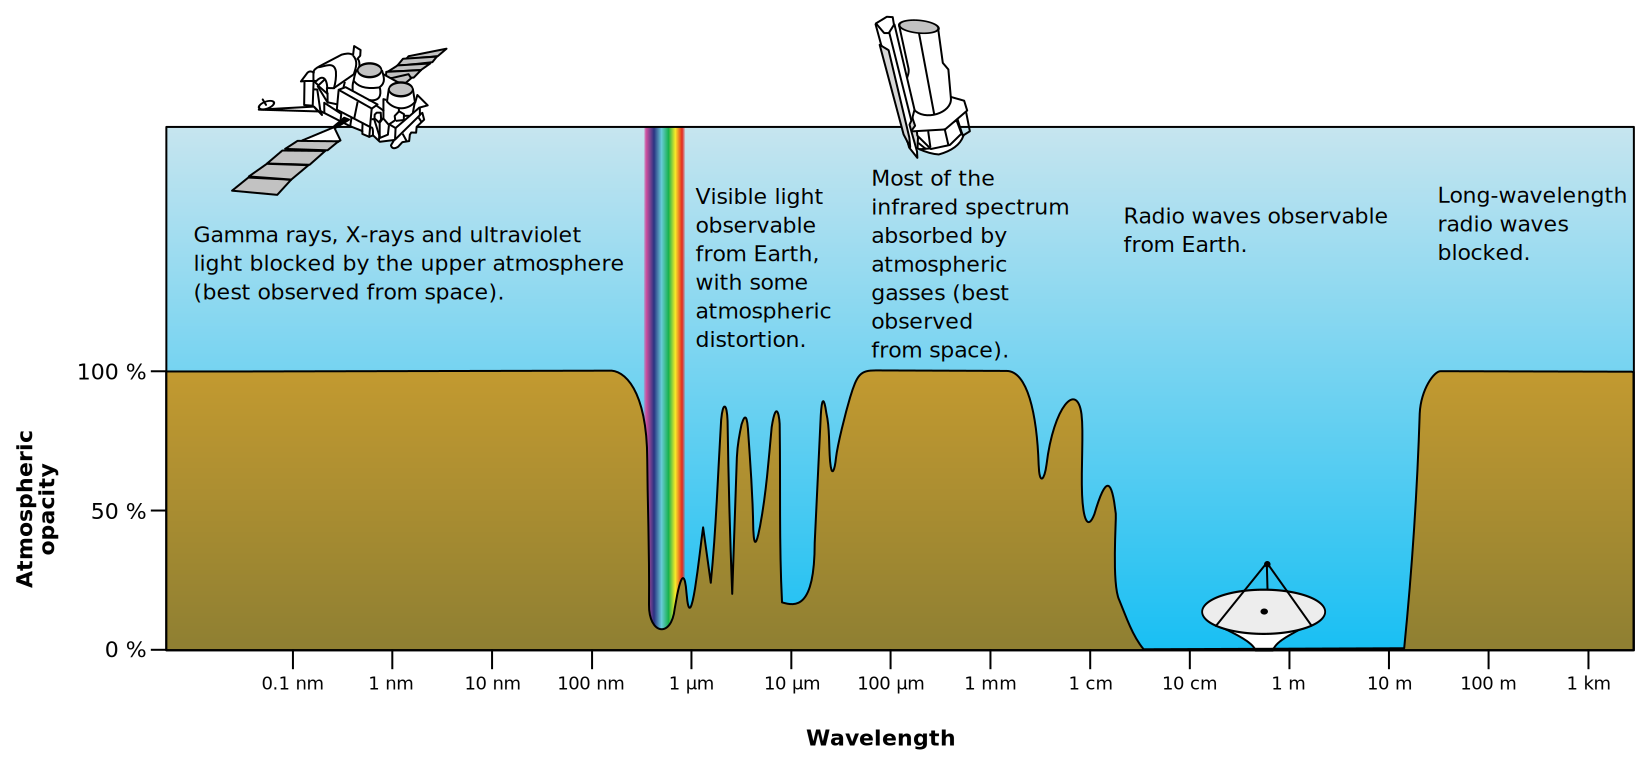
\includegraphics[width=\textwidth]{images/Atmospheric_electromagnetic_opacity}
\caption{Opacity of the Earth's atmosphere given different wavelength coming from space. Source \texttt{wikipedia}}
\label{fig:atmospheric-opacity}
\end{figure}

\begin{figure}[]
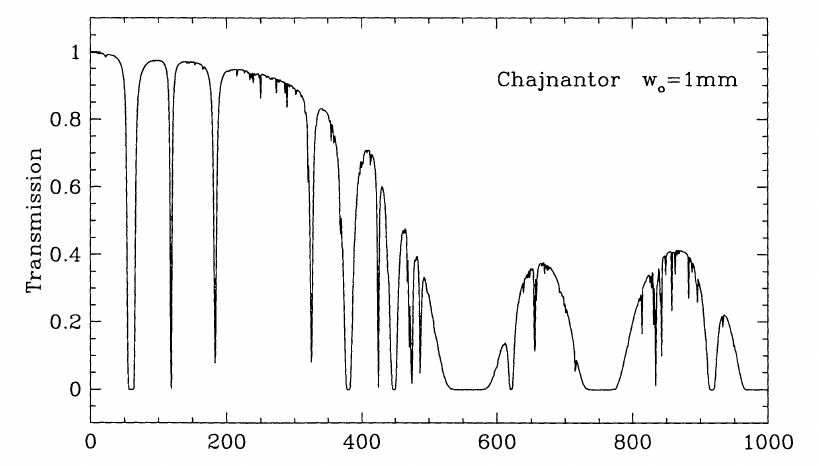
\includegraphics[width=\textwidth]{images/chajnantor-atm-transmission}
\caption{Transmission of the atmosphere from 0 to 1000 GHz for the ALMA site at Chajnantor in Chile assuming the typical value of $w_0 = 1 mm$ of precipitate water vapor. Source: \cite{taylor99}}
\label{fig:chaj-atm-tx}
\end{figure}

\begin{figure}[]
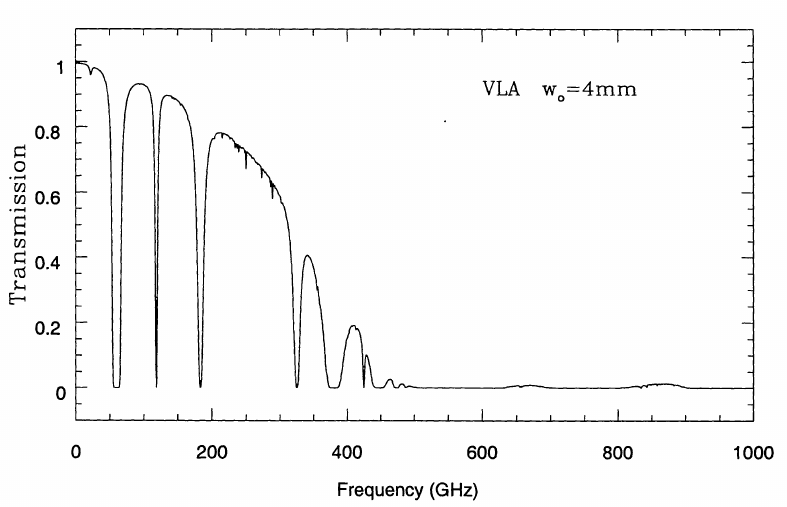
\includegraphics[width=\textwidth]{images/vla-atm-transmission}
\caption{Transmission of the atmosphere for VLA site in Socorro, NM, assuming a value of $w_0 = 4 mm$. Source: \cite{taylor99}}
\label{fig:vla-atm-tx}
\end{figure}

Figure \ref{fig:vla-atm-tx} shows the model of the atmospheric transmission at cm and mm wavelengths for the VLA site at 2150 m of altitude, figure \ref{fig:chaj-atm-tx} shows the model for ALMA site located in Chile at 4600 m of altitude. In both plots is possible to see a strong absorption lines including the water line at 22 GHz and 183 GHz, and the $O_2$ lines at 60 GHz and 118 GHz, plus a systematic decrease in the transmission with increasing frequency between lines. Every plot includes a different value for the column density of precipitable water vapor $w_0$ where each of one is typical for the site where the samples were taken. The precipitable water vapor (PWV) is the depth of the water vapor in the atmosphere in the site if it were converted to liquid phase.

Another important parameter in radio astronomy is the \textit{System Temperature ($T_{sys}$)}, this quantity measures the overall sensitivity of the receiving system. At centimetre, millimetre wavelengths, the temperature of the receiving system dominates the system noise temperature that is the receiver and the antenna. 

The calculation of $Tsys$ will be done in three steps:
\begin{enumerate}
\item First the Precipitable Water Vapor (PWV) content is determined. There are
several ways of doing this:
\begin{enumerate}
\item Calculate PWV from the Relative Humidity (RH) or the Dew Point. One way
of doing this is found in the MMA Memo No. 237, ``Precipitable Water at the VLA --
1990-1998'', by Bryan Butler. In this paper the PWV is developed as
$$
h = \frac{m_w P_0 H}{\rho_l k T_0}
$$
where $m_w$ is the mass of a water molecule (18 amu), $P_0$ is the water vapor
partial pressure, $H$ is the scale height of water vapor distribution (an
exponential distribution, 1.5 km for the VLA), $\rho_l$ is the density of
liquid water ($\mathrm{gr}/\mathrm{cm}^3$) and $k$ is the Boltzmann constant.

This memo presents a way to estimate $P_0$ from the dew point. In the subsequent
MMA Memo No. 238, ``Precipitable Water at KP -- 1993-1998'', a way of calculating
$P_0$ from the relative humidity is given:
$$
P_0 = 2.409 \times 10^{12} \ RH\ \theta^4 \exp(-22.67\theta)
$$
where $\theta$ is the inverse temperature ($\theta = 300/T_0 $ K), and $RH$ is
the relative humidity.

\item Calculate it from the opacity $\tau_{225}$ at 225 GHz measured by the
tipper. In this case a way of calculating the $PWV$ can be seen in
ALMA Memo 271 ``The Determination of Precipitable Water Vapour at Llano de
Chajnantor from Observations of the 183 GHz Water Line''. $PWV$ can be obtained
by inverting
$$
\tau_{225} = 6.7787\cdot 10^{-3} + 4.0757\cdot 10^{-2} PWV + 9.59\cdot 10^{-4} PVW^2
$$
\item Get the PWV directly from the Water Vapor Radiometers.
\end{enumerate}
When the $PWV$ is available from different sources, the different values
are averaged.

\item Interpolate the ATM tables to determine the opacity $\tau$ and the
atmospheric effective temperature $T_{atm}$. The ATM tables have the following structure:
\begin{eqnarray*}
\tau & = & \tau(\nu_i, PWV_j) \\
T_{atm} & = & T_{atm}(\nu_i, PWV_j)
\end{eqnarray*}
where $\nu_i$ covers the range $20-1000$ GHz with 100 MHz granularity, and $PWV_j$
covers the 7 values 0.4772, 0.658, 0.9134, 1.262, 1.796, 2.748, and 5.186 (mm). 
\item The system temperature is calculated as:

$$
T_{sys} = \frac {\left ( T_{rx} + T_{ant} + \xi T_{ant} \right ) e^{\tau / \sin(el)}}
{\eta}
$$
where $T_{rx}$ is the receiver temperature, $\eta$ is the forward efficiency (or
feed efficiency, or spillover factor), $T_{ant}$ is the antenna temperature and $\xi$
is the sideband ratio, which for practical purposes will be $0$

Expanding the calculation of above:

$$
T_{sys} = \frac{\left ( T_{rx} + \eta T_{atm} \left ( 1 - e^{-\tau/\sin(el)} \right ) + (1 - \eta) 0.95 T_{amb} + \eta 2.76 e^{-\tau/\sin(el)} \right )  e^{\tau / \sin(el)}}
{\eta}
$$
where $T_{amb}$ is the ambient temperature, which is read from weather station.
\end{enumerate}


\section{ALMA Project Data Model}
\label{sec:apdm}
The ALMA Software system works using the concept of an Observing Project, the full description and the details of the model are available at~\cite{apdm-model}. The Observing Project is used throughout the ALMA software as the top level structure associated with a project resulting from a single observing proposal. In fact the Observing Project is a container for all the information relating to a project before it begins execution. During and following execution other data associated with the project are created and held in other structures, each of which holds a reference to the original observing project. Of particular interest is the Project Status structure, which holds a record of the execution status of the Project. The ALMA Project Data Model (APDM) defines the structure of both the Observing Project (ObsProject) and the execution status (ProjectStatus).

The Scheduling Block (SchedBlock or SB) is the atomic unit of observing for ALMA, any given science observation will usually be broken into many SBs, which may, or may not be executed in sequence. The ALMA Scheduling Software will decide on which SB to execute at any given time on the basis of which is the best to execute now. An SB as a canonical execution length of around 30 minutes, however in practice the SBs observation duration could be up to 2 hours, depending of the Observation program.

\begin{description}
\item[Observation Project Entity] \hfill \\
When a ALMA user submits a project to the Data Base, then the user is creating a ObsProject. Almost all the end-user tools in ALMA operates on ObsProjects, no other entities are exposed to the end user.

In order to hold all of the pre-observing information associated with a project the ObsProject entity class is composed of three parts: an ObsProposal, an ObsReview and an ObsProgram. These hold the information associated with the three phases of observing preparation: the proposal or Phase I, the reviewing and resultant approvals, and the observing program definition, or Phase II.

\item[Observation Program Entity] \hfill \\
The Observing Program (ObsProgram) part of the Observing Project holds all the information created during Phase II, or program preparation. The ObsProgram consists of an Observing Plan (ObsPlan) and a SciencePlan. The Science Plan covers the science goal oriented view of the observing, and it is intended to contain the information that most users will use to define their observing programs. This information will persist, for the convenience of users, but will not be the definition that is used by the Observatory when carrying out the observations. Instead the latter information is contained within the ObsPlan, and covers what we call the system view. The service of Program Generation allows users to create the Observing Plan from their Science Plan. It is also possible for very advanced users to ignore the Science Plan and simply create all of the Observing Plan directly.

As stated, the Observing Plan (ObsPlan) is the container for defining the actual observing objects. In modeling terms the ObsPlan is a role for the top level ObsUnitSet, heading the definition of the system view. An ObsUnitSet contains a collection of Scheduling Blocks or more ObsUnitSets, along with objects defining the preconditions, performance and calibration requirements, and flow control that apply to that collection.


\item[Scheduling Block Entity] \hfill \\
A Scheduling Block (SB) is the unit of observing for ALMA. It defines all the information that is required by the Observatory to independently execute the acquisition of a set of data and then to calibrate it as well. Since SBs are selected for execution individually they must exist as separate items in the data base.

Most of the structures within the SB hold information that is used either by the scheduler, to query whether or not this SB is suitable for scheduling ``now'', or as information that is used by the Observing Script (in the Control subsystem) to actually execute the observing (see below), and in some cases both. There are also performance goals for the SBs, to be measured against by the observing system.

So to allow the determination of ``Schedulability'' we find items like representative target observability, weather constraints, a precondition that requires a current Baseline Calibration and a Scientific Priority.

\item[Targets] \hfill \\
The target is the element within an SB that defines the area to map, the spectral or instrumental setups to use, and the purpose of the observing. In fact the target element itself contains nothing except references to other elements that contain descriptions of these three key components.

\end{description}

\section{General problem}
\newtheorem{problem-def}{Definition}
The atomic unit to be scheduled is called scheduling block, this name matches the name described in section~\ref{sec:apdm}, although it differs since, the scheduling block is defined as atomic unit here, it contains only one target, the \textit{representative target}, which is the most representative of the set of targets for the given scheduling block. The submitter of the proposal is in charge to choose the representative target.


\begin{problem-def}
A Scheduling Block (SB) is represented as a n-tuple of time independent  properties ($P$). Let $S_0$ be the set of all SBs,
$$S_0 = P_1 \times P_2 \times ... \times P_n,$$
for appropriate $P_i$ sets. Then one SB is:
$$sb = (p_1, p_2, ..., p_n) \mid p_i \in P_i$$
\end{problem-def} 

Once defined a scheduling block, then the operation of selecting SB can be defined as:
\begin{problem-def}
The scheduling blocks selection is represented as a function that for a given time $t$ and a set of SBs $S \subseteq S_0$, it returns a subset of S:
$$sel:(t,S) \rightarrow \mathcal P \left({S}\right)$$
\end{problem-def}

Given these definitions, a property of $sel$ follow:

\newtheorem{sel-props}{Property}
\begin{sel-props}
The full selection operation $sel$ for a given time $t$ can be decomposed in independent selection operations, one for each property $p_i$:
$$sel(t,S) = sel_1(t, S) \cap sel_2(t, S) \cap ... \cap sel_n(t,S)$$
In general, each one of these selection operations can be expressed  as an inequality, defining the ``schedulable time window'' for a given $sb_j$:
$$sb_j \in sel_i(t, S)\,i.i.f\;\alpha_1(t, sb) \leq \alpha(t, sb) \leq \alpha_2(t, sb)$$
\end{sel-props}

Without losing generality, the inequality of the property of above can be separated in two inequalities, then the condition can be expressed as: 
$$\alpha'(t, sb) \leq \alpha (t, sb)$$
Regarding the dependencies of both $\alpha$ and $\alpha'$, if the property depends on $t$, then the property is \textit{dynamic}, which means that the property value to satisfy the inequality is calculated and updated accordingly the scheduling algorithm progress. In other hand the properties depending only on $sb$ are \textit{static}, therefore the values to satisfy their inequalities are pre-calculated at the beginning of the algorithm.\\

\subsection{Static an dynamic constraints}

As stated in section~\ref{sec:apdm} a target is composed by three elements, which match the constraint categories detailed here: \textit{sky source}, \textit{instrumentation} and \textit{weather}.

In common terms a Scheduling Block is ``schedulable'' only if the representative target for the given scheduling block is observable, this means that the source of the sky is visible, the array configuration has enough hardware capabilities to observe the source according to the scientific plan, the weather conditions are good enough to carry on the observation, etc. Basically this is the intersection of the different $sel$ functions and it is defined as the \textit{schedulable time window} for a given scheduling block, this window could be available several times during the observing season. In practical terms a scheduling block can be observed as many times as possible until it has been complete.

The description of each one of the different categories is as follow:

\begin{description}
    \item[Instrumentation] \hfill \\
Every scheduling block execution is done in an \textit{Array} which is a subset of the available antennas in the observatory. Each antenna has its own hardware configuration to receive electromagnetic waves from the space. An array will have the hardware configuration common to all the antennas conforming the array, the idea is to observe the target with the same hardware in all the antennas as they were a single instrument. In general, in an observatory all the antennas conforming an array will have all the same capabilities, even they can be interchange each other and should not be any difference. The array configuration and the availability of the instrumentation is decided beforehand and for effects of the algorithm is considered an static constraint. 

Nonetheless, problems in some instruments during observatory operations could temporally remove some capabilities from some antennas, or even the entire antenna could be removed, altering the original instrumentation properties that the array was given initially. Since all these failure are not planned this is considered a dynamic constraint.

	\item[Sky source] \hfill \\
In general a sky source will be visible in daily basis for certain amount of time, then the source will go below horizon due the Earth's rotation, unless the source is circumpolar in which case the source will be always visible. Also the Earth's orbit movement around the sun would cause that a source will be visible during a period of the calendar year only. Both of these source properties are predictable and can be calculated before the execution of any observation.

Every time that a observation starts, the telescope needs to be calibrated to adjust pointing corrections based on atmospheric conditions and source position. It is possible to predict how much time will be spent on calibrations if the observation plan is given before the execution of observations starts, however sometimes this is not the case due improvement or deterioration of weather conditions expected, making this constraint dependable on the time the observation being executed.
  
	\item[Weather] \hfill \\
The weather cannot be foreseen with exactitude, even the most accurate weather forecast will have a error margin, which will increase if the period of time foresaw increase. Once the weather condition has changed, for good or bad, usually the list of the scheduling blocks to be observed needs to be updated accordingly. The time frame on what the algorithm can optimize the observations is bounded to the reliability of the weather pattern prediction, doing optimizations beyond that could be worthless.

\end{description}

Another important property of every project submitted to be observed in the observing season, is that they does not have the same science value, this means there are certain projects that are more interesting to observe and complete than others. This measure of how much value has a project is given by science team of the observatory, therefore the scheduler must be aware of this and try to complete most of the projects having the ``highest'' science qualification, this will be known as the \textit{scientific throughput}.

\subsection{Completing Scheduling Blocks and Observation projects}
\label{subsec:completing-obs}
A scheduling block does not need to be completed in just one observation, in fact the scheduling block cn be observed multiples times at different time, hence different weather conditions and different array configurations, until the scheduling block is considered complete.
A scheduling block will be completed, and put its state as complete, if it meets any of following three criterion:
\begin{itemize}
	\item \textit{Number of repetitions}: A scheduling block could have a limit of how many times can be observed.
	\item \textit{Total time observed}: A scheduling block could have a limit of how much time can be observed.
	\item \textit{Sensitivity achieved}: As stated in section \ref{sec:sens} if the goal for the RMS noise accumulated is achieved, then the scheduling block will be considered completed.
\end{itemize} 
Some of the scheduling blocks could not have all the three criteria, it is enough for the SB to have a least one of them.

The criteria to determine if a project was complete, is based in how many scheduling blocks or ObsUnit sets have been completed, or the total amount of time observed, which is the sum of all the scheduling blocks observations. However, in reality human intervention is required to determine if the project has been completed based on the quality of science data extracted from the observations. The algorithm establishing whether a Observation project is completed or not is far beyond the scope of this study. 

\subsection{Observing season (Observation cycle)}
Until this point, this study has tried to explain and referred only to observation properties within the time frame considering only one instrument (just one instrument spawns for the whole observation time frame). 

However, over the whole time available in the observing season, it is possible to have different \textit{Array configurations}, that can co-exist at the very same time with other array configurations, or can be created in serial over the time frame of the observation season, or a combination of both situations.

Each array configuration can be composed of 1 or more antennas available at the observatory, each one can offer different science capabilities, which can be or cannot be used by the scheduling block, nonetheless each array will offer basic differences like the $uv$ coverage as seen in section \ref{sec:uvcover}, the angular resolution explained in section \ref{sec:angular-res} or the sensitivity achieved in every observation (section \ref{sec:sens}), which is dependent of the number of antennas in the array. As well one or more arrays can be available for observations at the same time as said before, however each scheduling block must be observed by just one array at a given time.

\subsection{Identified problems}
\label{sec:problems}
After the analysis of the different properties and constraints related to the astronomy scheduling problem it is possible to identify the following two different problems:
\begin{description}

\item[Scheduling array problem] \hfill \\
The \textit{scheduling array problem} consists on determine a schedule for a given set of scheduling blocks, which all of them can be observed by the instrument, considering one array already created within a given period of time. 
The idea is to generate a plan to try to observe all, or most of the projects with the highest scientific value in the less amount of time possible considering all, or the most critical of the scientific requirements. It may possible to not complete all the observation projects submitted for this array configuration. Slso is desirable to reduce the amount of idle time of the instrument.

\item[Array configuration schedule problem]

The \textit{array configuration schedule problem} is on top of the scheduling array problem. It consists in try to determine a schedule of observations, for the observing season (which is a fixed amount of time and it lasts for several months, up to a couple of years), for a given set of the scheduling blocks and a given set the array configurations. The idea is to try to observe most of the projects with high scientific value considering all, or most of the scientific requirements during the observing season, however not all the observation projects may not be completed. Also it is desirable to reduce the idle time of the observatory as whole.
\end{description}


\section{ALMA Scheduling Problem}
\label{sec:alma-sched-problem}
The Atacama Large Millimeter/submillimeter Array (ALMA) is a major collaboration effort between European, North American and East Asian countries, under construction on the Chilean Chajnantor plateau, at 5.000 meters altitude. When completed in 2013 it will be the largest radio telescope on earth, with more than 60 antennas of 12 and 7 meters diameter, distributed over a wide extension, with up to 16 kilo-meters of baseline separation. The ALMA interferometer will provide the possibility to be used as a single array, or as up to six (due to limited centralized equipment, photonic references) minor independent arrays or groups of antennas. As each array is equivalent to one instrument, this can eventually be seen as a multi-telescope problem. Also, the antennas will be changing their positions over the year, as different distributions will be used to exploit various kinds of observations. As ALMA does not observe in the visible spectrum, observations are not limited to night time only, thus a 24/7 operation with as small downtime as possible is expected. 

ALMA will operate exclusively in service mode. Therefore, the Scheduling software Subsystem is supposed to provide a fully automatic “quasi-real-time” dynamic scheduling platform, mostly with the only human participation of supervision. This Subsystem is still under development, and the needed algorithm(s) are still in a preliminary state. The main problem is the dynamic priorities scheduling, which differs widely from the traditional dynamic job-shop. This particular problem is very similar for all ground based observatories, and ALMA is one real example, that needs this kind of scheduling to accomplish its operations requirements.

The ALMA telescope will be operated as one or more antenna arrays, executing observation blocks corresponding to accepted project proposals. There will be three different antenna types, provided by three vendors:
\begin{itemize}
\item 12-m antennas (50): This is the main array to be operated, and also the one to be divided into several sub-arrays. They are provided by vendors Vertex (Vertex Antennatechnik GmbH) and AEM (Alcatel Alenia Space France, Alcatel Alenia Space Italy, European Industrial Engineering S.r.L., MT Aerospace).

\item 7-m antennas (12): This is the main part of the ALMA Compact Array (ACA), which will  operate as a separate array. They are provided by MElCo (Mitsubishi Electric Corporation).

\item 12-m total power antennas (4): These are special total power antennas able to see a full 2GHz spectrum, part of the ACA, but in principle exchangeable with any of the other 12-m antennas. They are also delivered by MElCo.

\end{itemize}

\begin{figure}	
\begin{center}
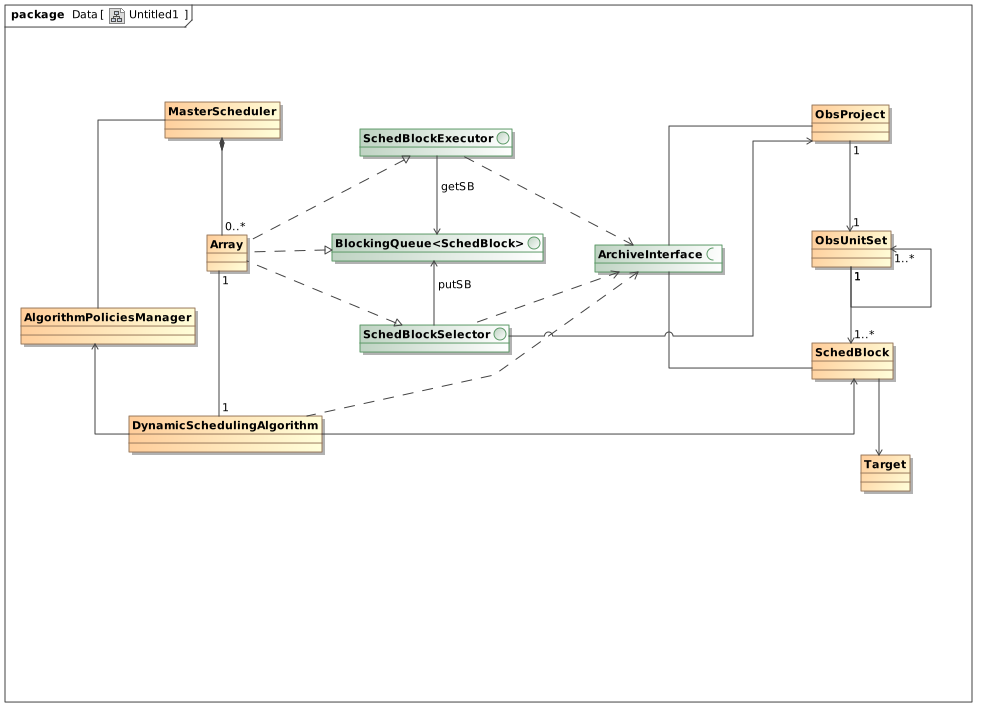
\includegraphics[width=\textwidth]{images/scheduling_class_model}
\caption{Basic class model of Scheduling subsystem.}
\end{center}
 \texttt{MasterScheduler} and \texttt{Array} are the common classes used by all kind of Arrays. \texttt{DynamicSchedulingAlgorithm} is the class implemenenting the current ALMA's dynamic algorithm. At right side of the figure it is available the hierarchy of the the top level APDM classes used by the scheduling subsystem, which are accessed through the \texttt{ArchiveInterface}.
\label{fig:sched-class-model}
\end{figure}

A huge part of the telescope operations will be handled through the ALMA software, which is divided into various subsystems, such as Control, Correlator (ACA and Baseline), Pipeline, Archive, Scheduling and Offline software. The big picture of ALMA Software can be seen in~\cite{schwarz04}.
The Scheduling Subsystem is the one in charge of managing antenna arrays and dynamically executing scheduling blocks. The current software design details are in~\cite{clarke12}. The basic design considers 4 main parts which are represented in figure \ref{fig:sched-class-model}: The ``Master Scheduler'', The ``Array'', The ``Dynamic Scheduler instance'' and the ``Archive Interface''. The Master Scheduler is in charge of create and manage the creation of the Arrays and handle the management of the Scheduling Policies to be used in the DSA. The Array is the main operations unit of the scheduling subsystem, each array operates over Scheduling Blocks, executing, waiting for results of the observations and notifying to the user of the system what has been the outcome of the observation. The Array uses directly the Archive, which is the database storing the definition of each Observation project (see~\ref{sec:apdm}), through the Archive Interface. Each array has its own scheduling queue, which can contain several schedblocks waiting to be executed, but just one SchedBlock is observed at the same time in each Array. Finally the DSA acts as a component of an Array selecting the current best SB according to the algorithm policy selected for the given Array, the details of the ALMA's DSA is discussed in section \ref{sec:alma-dsa}. Additionally each scheduling array can operate in 3 different modes: Manual, in this mode the scheduling queue is set with a maximum of one item, in this mode the user is responsible to execute the observation manually using low level scripts. Automatic, in this mode the array has a unlimited size scheduling queue, once a observation has been completed a new SchedBlock is taken from this queue to observe the next one until the queue is empty or the scheduler is stopped. And Dynamic, in dynamic mode the scheduling queue behaves as the array in interactive mode, but when the queue is empty the DSA is triggered selecting the next best SchedBlock to observe, depending if the DSA is active or passive the selected SchedBlock will be put in the queue to start the observation or the Scheduler will notify the user only respectively. The state machine implemented as part of the current DSA can be seen in the figure~\ref{fig:sched-dsa-state-machine}, the DSA may be executed every time that a new Scheduling Block is needed to be queued, until there is no more Scheduling Blocks available.

\begin{figure}	
\begin{center}
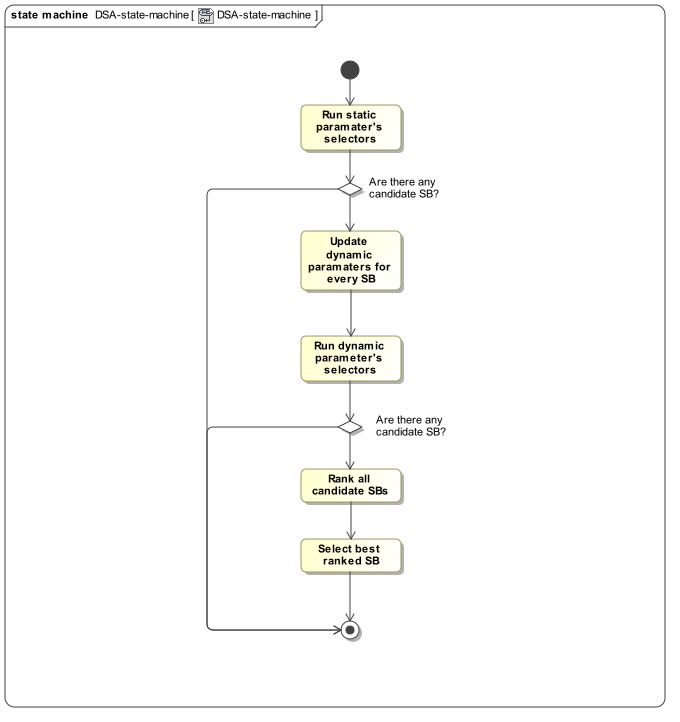
\includegraphics[width=0.9\textwidth]{images/DSA-state-machine}
\caption{Dynamic scheduling algorithm's state machine}
\end{center}
\label{fig:sched-dsa-state-machine}
\end{figure}


It is true that most of the scheduling software will be run in the on-line software, however there is a planning stage where the Scheduling algorithm will contribute to plan different scenarios within a season. The on-line usage of the algorithm is known as the \textit{short-term scheduler}, this scheduler either can be used in quasi-real time or to planning the night observations. A \textit{medium-term scheduler} used to planning the observations of a frame of time where the array configurations are the same. And finally \textit{long-term scheduler} which should be able to plan an entire season of observation across the different planned array configurations, ideally the algorithm should define the duration of each configuration given as a input. For the two last use cases a ALMA scientific operations uses a simulator, which are mostly described in~\cite{hoffstadt10}. Although new features have been added, the basic workflow has been kept until now.